\documentclass[12pt]{article}
\usepackage{graphicx}
\usepackage{fullpage}
\usepackage[tikz]{bclogo}
\usepackage{fancybox}
\usepackage{amsmath,hyperref,color,clrscode,graphicx}
\begin{document}
\centerline{\bf Homework 3 - CSE 276 - Math for Robotics}
\centerline{Due: 4 November 2021}

\begin{enumerate}
\item In the following circuit, $V=10^3 sin{\sqrt{\pi t}}$, $R_1=1k\Omega$ and $C_1=2mF$. The parameter $q$ is considered as electrical charge for capacitor $c_1$. If $q(0)=4C$ and $h=0.1$, determine $q(t)$ at $t=0.1$ using the following methods:

\begin{enumerate} 
	\item Euler's Method
	%\item $2^{nd}$  Order Runge-Kutta's Method (Modified Euler)
	%\item $3^{rd}$ Order Runge-Kutta's Method
	\item $4^{th}$ Order Runge-Kutta's Method
	%\item Calculate the exact answer and explain your conclusion.
\end{enumerate}
 (hint: Write KVL and simplify it: $V-IR-\frac{q}{C}=0 \to I=\frac{V}{R}-\frac{q}{RC} \to \frac{dq(t)}{dt}=\frac{V}{R}-\frac{q}{RC}$)
\begin{center}
 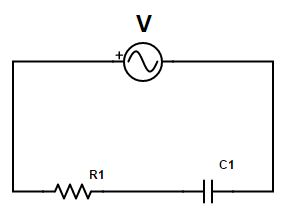
\includegraphics[scale=1.0]{Capture}
\end{center}

%%%%%%
 
 \item Let $X$ be a random variable with probability density function (PDF) $f(x)$, as defined below:
$$
f_X(x) = \begin{cases}
\frac{1}{e}\left [e^x(x+1)\right] \text{\hspace{0.5cm} if } x \in [0, 1] \\
\text{0 \hspace{1cm} otherwise}\\
\end{cases}
$$
Find the expected value of X, $\mathbf{E}[x]$, by ($h = 0.1$):
\\
\begin{enumerate}
\item Rectangular method
\item Midpoint method
\item Trapezoidal method
\end{enumerate}
 

 
%%%%%%%% 
\item Consider the following differential equation over the interval
  $(0, 1]$:
\[
\frac{dy}{dx} = \frac{1}{x^2(1-y)}
\]
with y(1) = -1. 

\begin{itemize}
\item Obtain an exact analytical solution to the equation

In the following solve for y(0) even though in theory the equation is
not defined for x=0. 

\item Implement and use Euler’s method to solve the differential
  equation numerically. Use a step size of 0.05. How accurate is your
  numerical solution?

\item Implement and use a fourth-order Runge-Kutta method to solve the
  differential equation numerically. Again, use a step size of
  0.05. Again, how accurate is your numerical solution? 

\item Implement and use a Richardson extrapolation to solve the
  equation, again with a step size of 0.05. How accuracy is your
  solution compared to the analytical solution? 
\end{itemize}

\item We have multiple robots that can generate point clouds such as
  those coming from a RealSense camera. In many cases we want to use the 
  robots to detect objects in its enviroment. We provide three data
  files:
  \begin{enumerate}
  \item Empty-Table.pcd which containts a data for an empty table
  \item Cluttered-Table.pcd contains point cloud for a cluttered table
  \item Hallway.pcd contains data from a hallway
  \end{enumerate}
  Each file has the point cloud file in a format with each line
  contains $x_i ~ y_i ~ z_i$. 
  \begin{itemize}
  \item Provide a method to estimate the plane parameter for the
    table. Test it both with the empty and cluttered table. Describe
    how you filter out the data from the objects. You have to be able
    to estimate the table parameters in the presence of clutter. 
  \item Describe and show how the method can be generalized to extract
    all the dominant planes in a relatively empty hallway. 
  \end{itemize}
\end{enumerate}

\end{document}

%%% Local Variables:
%%% mode: latex
%%% TeX-master: t
%%% End:
